% !TEX root = ../main.tex
\chapter[Implementação e apresentação do sistema]{Implementação e apresentação do sistema}
\label{chap:implementacao-sistema}

Este capítulo apresenta uma seleção de telas do FlashFood, organizada conforme as áreas e os perfis de usuário. As figuras ilustram funcionalidades relacionadas aos requisitos correspondentes, mas não abrangem todos eles. Assim, a ausência de uma captura para determinado requisito indica apenas que ele não foi ilustrado nesta seção e, por si só, não permite concluir que não tenha sido implementado.

\section{Telas de acesso e cadastro}

A Figura~\ref{fig:acesso-cadastro} reúne a tela de \textit{login}, utilizada por usuários cadastrados conforme o RF02, e a tela de cadastro, destinada ao visitante que cria uma conta de cliente conforme o RF01. A tela de \textit{login} também apresenta o acesso à recuperação de senha.

\begin{figure}[H]
  \centering
  \caption{Telas de acesso e cadastro do FlashFood: (a) \textit{login}; (b) cadastro de usuário}
  \label{fig:acesso-cadastro}
  \begin{minipage}{0.9\textwidth}
    \centering
    
\includegraphics[width=\linewidth,height=0.29\textheight,keepaspectratio]{FlashfoodImagemSistema/login.png}
    \par\small (a)
  \end{minipage}
  \par\vspace{0.5em}
  \begin{minipage}{0.9\textwidth}
    \centering
    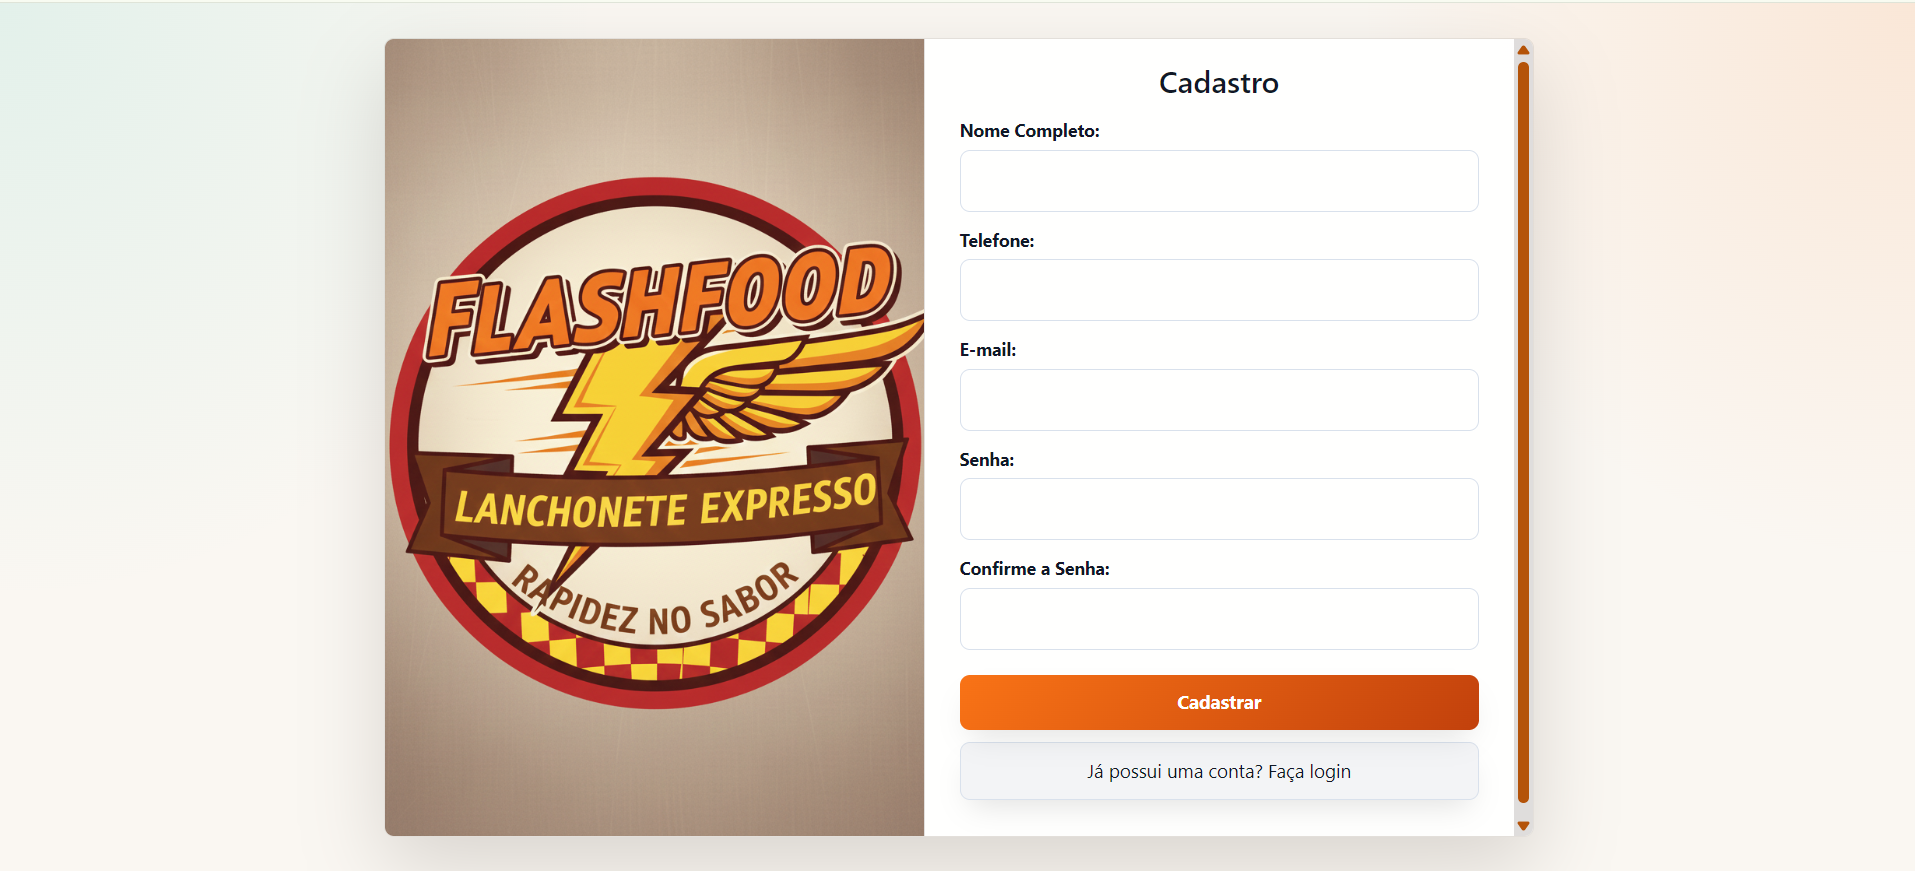
\includegraphics[width=\linewidth,height=0.29\textheight,keepaspectratio]{figuras/captura-cadastro-usuario.png}
    \par\small (b)
  \end{minipage}
  \legend{Elaborado pelo autor (2026)}
\end{figure}

\section{Área do cliente}

A Figura~\ref{fig:cardapio-cliente} apresenta a tela inicial da área do cliente, com a exibição dos produtos disponíveis para consulta. Essa tela atende ao RF05.

\begin{figure}[H]
  \centering
  \caption{Cardápio na área do cliente}
  \label{fig:cardapio-cliente}
  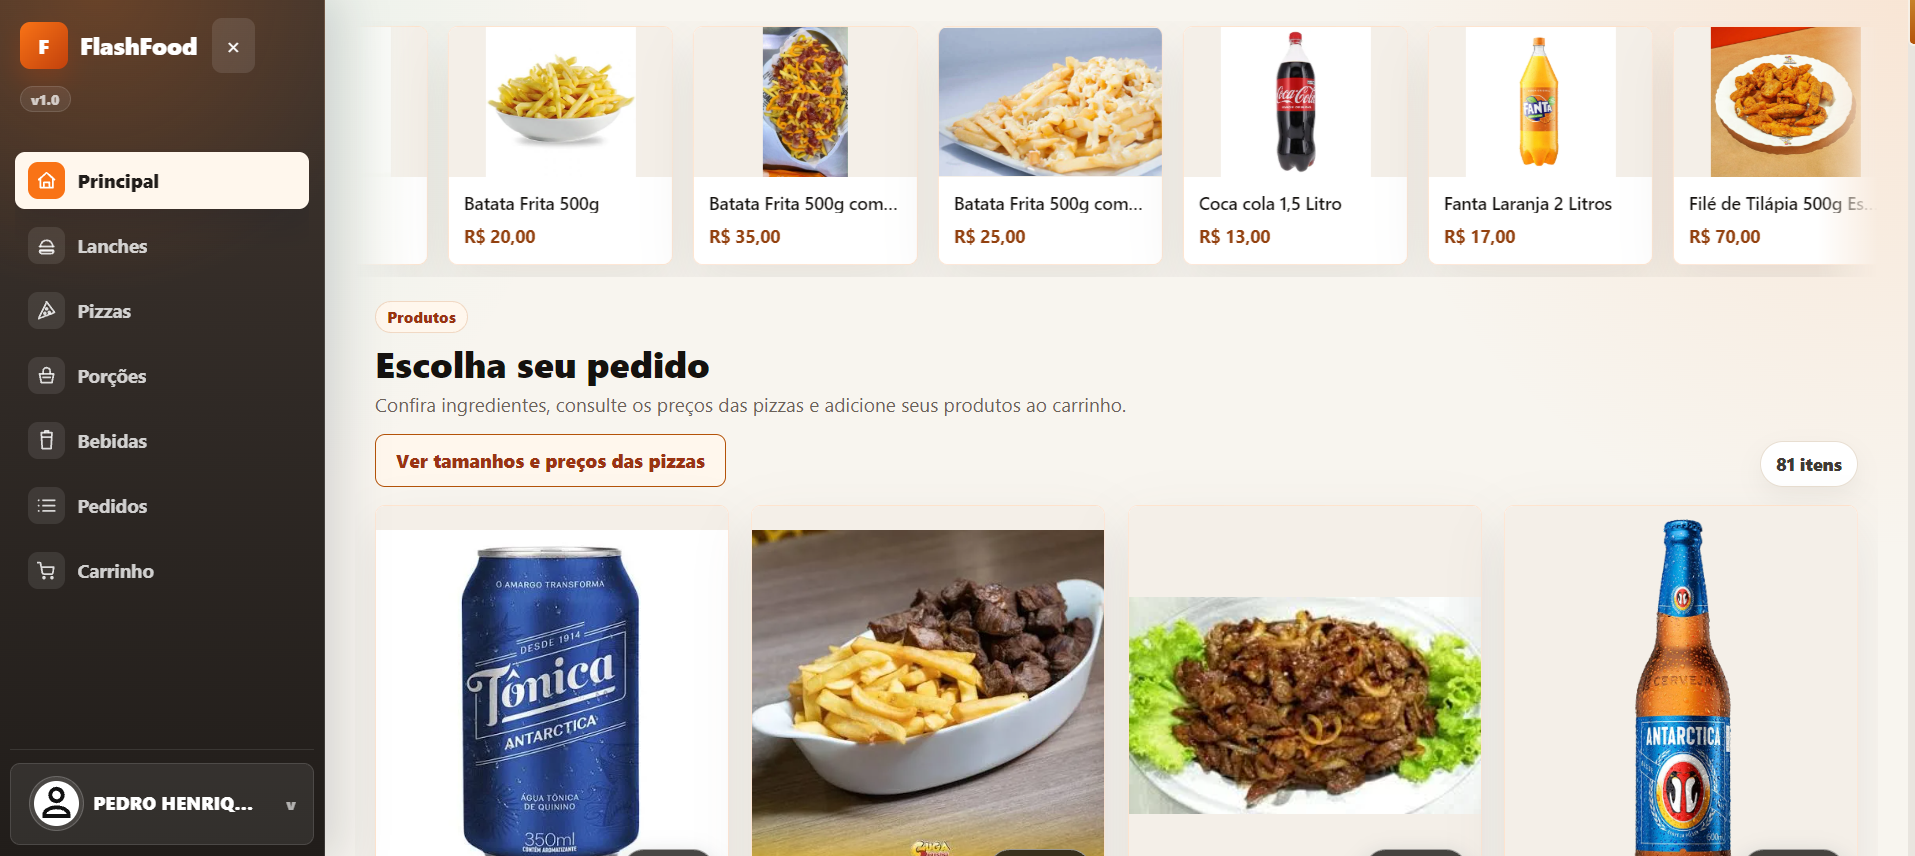
\includegraphics[width=\textwidth,height=0.68\textheight,keepaspectratio]{FlashfoodImagemSistema/telainicialCLinete.png}
  \legend{Elaborado pelo autor (2026)}
\end{figure}

A Figura~\ref{fig:carrinho-cliente} mostra o carrinho com um produto selecionado, sua quantidade e os valores correspondentes. A tela é utilizada pelo cliente no gerenciamento do carrinho, conforme o RF06.

\begin{figure}[H]
  \centering
  \caption{Carrinho de compras do FlashFood}
  \label{fig:carrinho-cliente}
  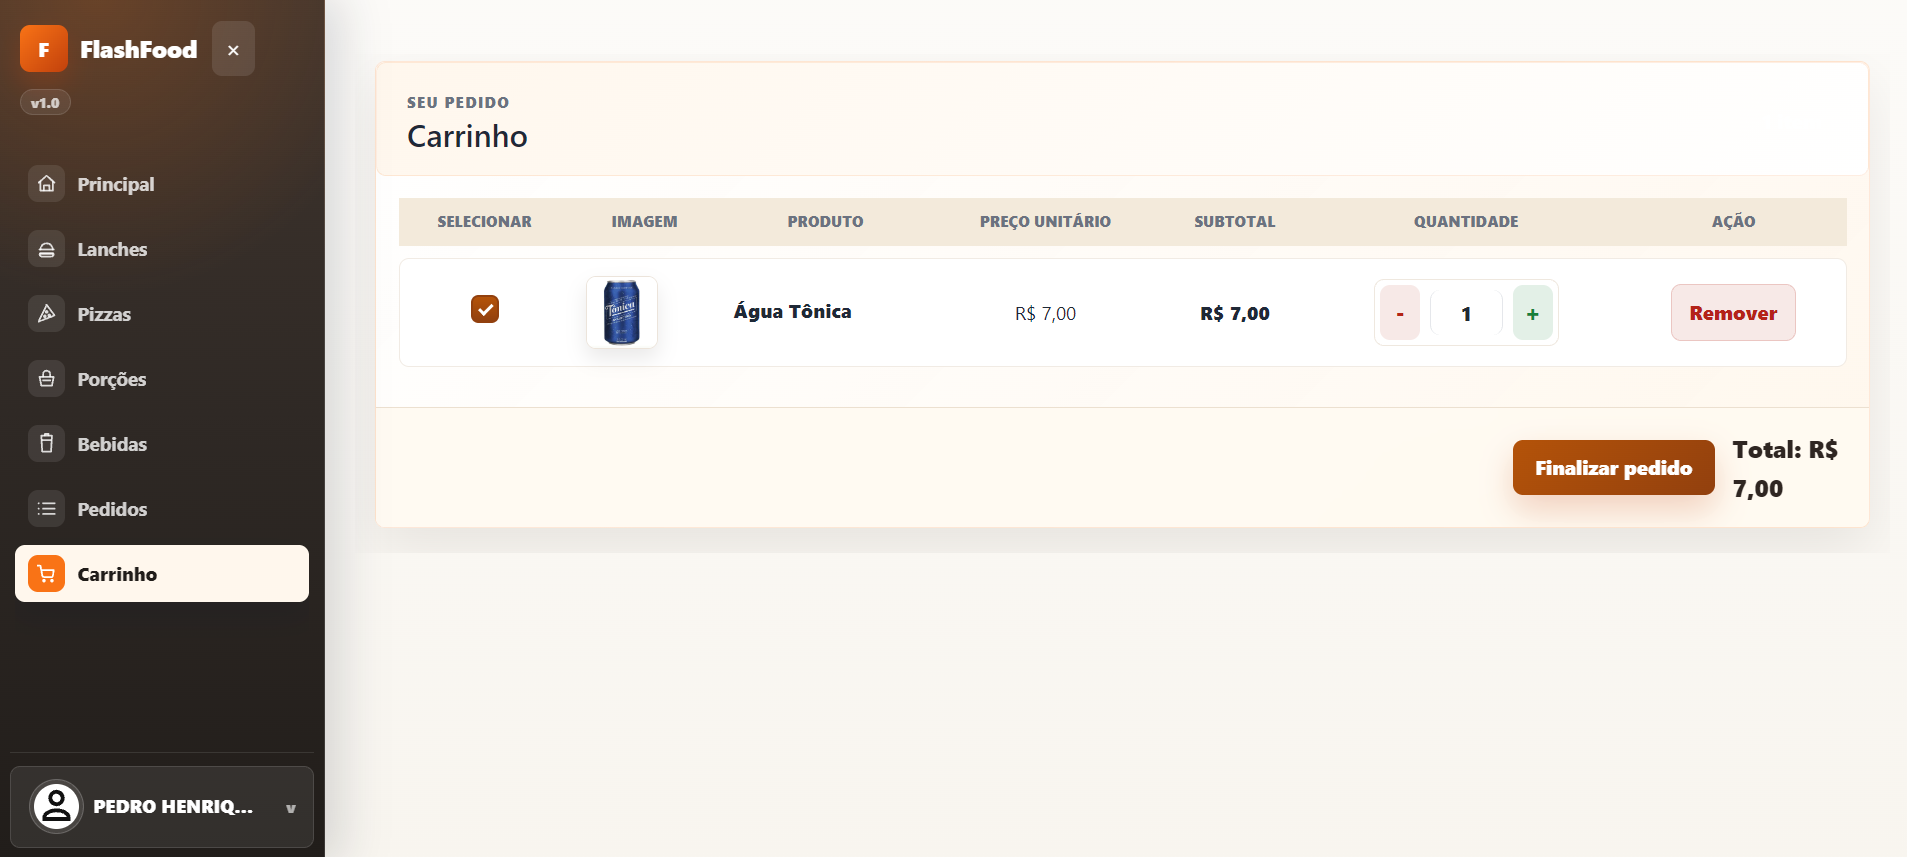
\includegraphics[width=\textwidth,height=0.68\textheight,keepaspectratio]{FlashfoodImagemSistema/carrinho.png}
  \legend{Elaborado pelo autor (2026)}
\end{figure}

\section{Área do administrador}

A Figura~\ref{fig:painel-administrador} apresenta o painel identificado na própria tela como área do administrador, com referências às áreas de pedidos, produtos e mesas. O controle de acesso por perfil relaciona-se ao RF03.

\begin{figure}[H]
  \centering
  \caption{Painel administrativo do FlashFood}
  \label{fig:painel-administrador}
  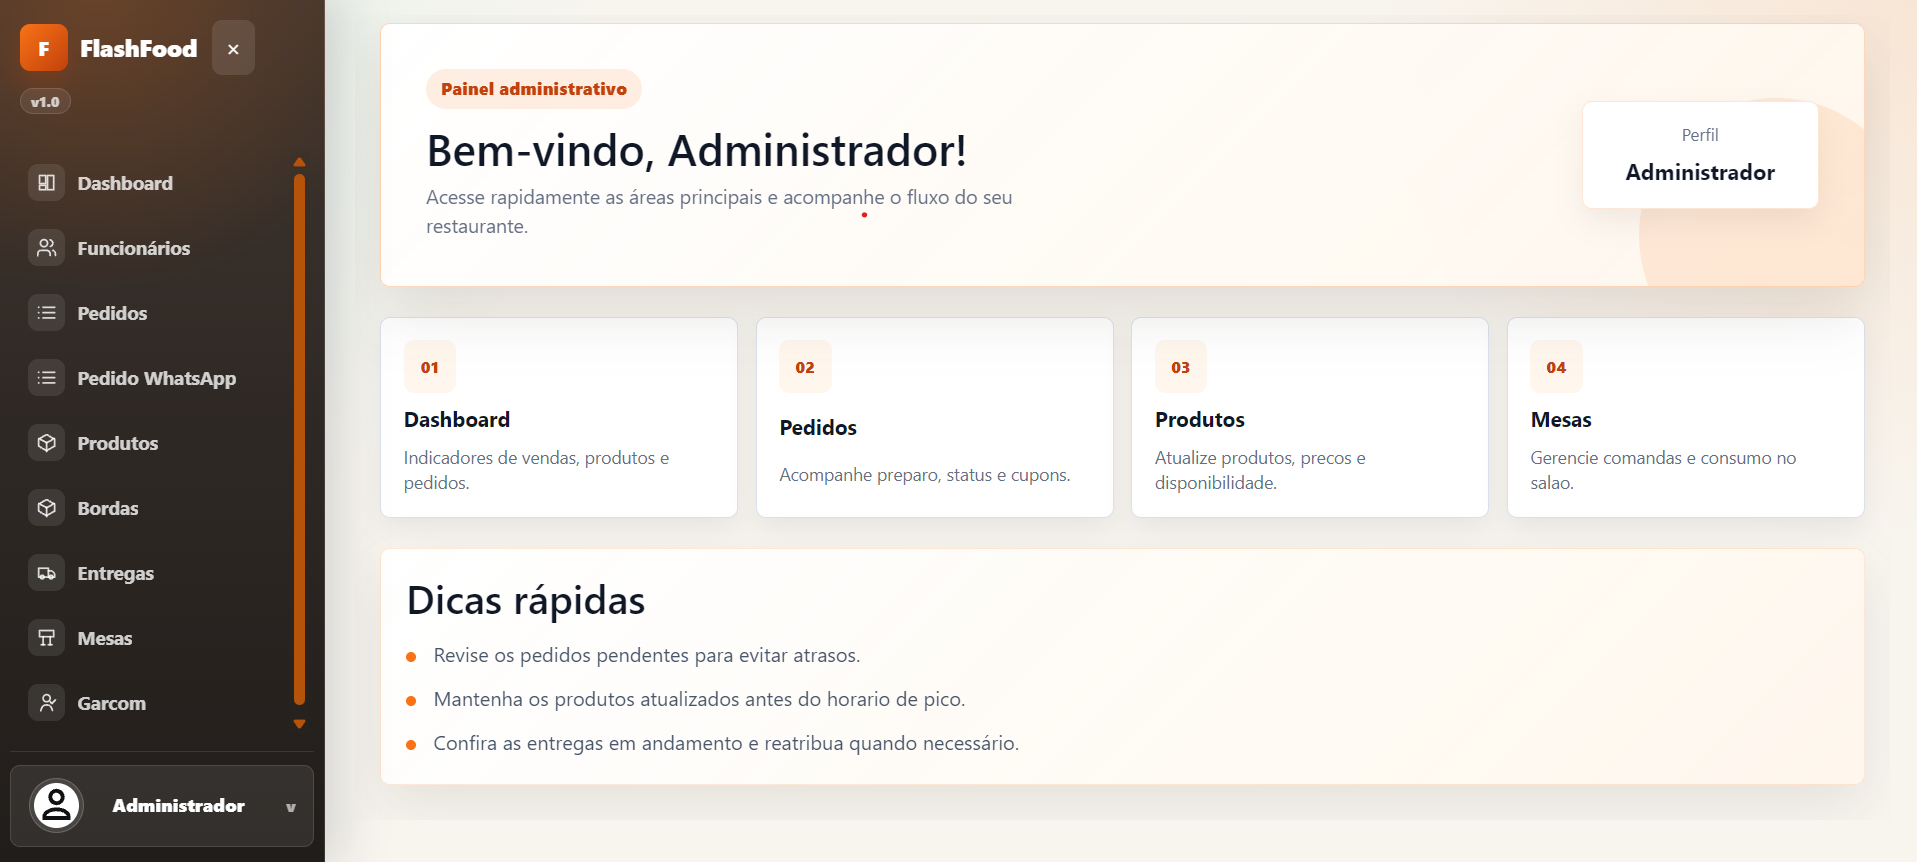
\includegraphics[width=\textwidth,height=0.68\textheight,keepaspectratio]{FlashfoodImagemSistema/telaadministrador.png}
  \legend{Elaborado pelo autor (2026)}
\end{figure}

A Figura~\ref{fig:produtos-administrador} apresenta a área de produtos, com a listagem e os dados associados aos itens cadastrados. Essa tela administrativa relaciona-se ao RF03 pelo perfil de acesso e ao RF11 pelo armazenamento e recuperação de dados de produtos.

\begin{figure}[H]
  \centering
  \caption{Gerenciamento de produtos pelo administrador}
  \label{fig:produtos-administrador}
  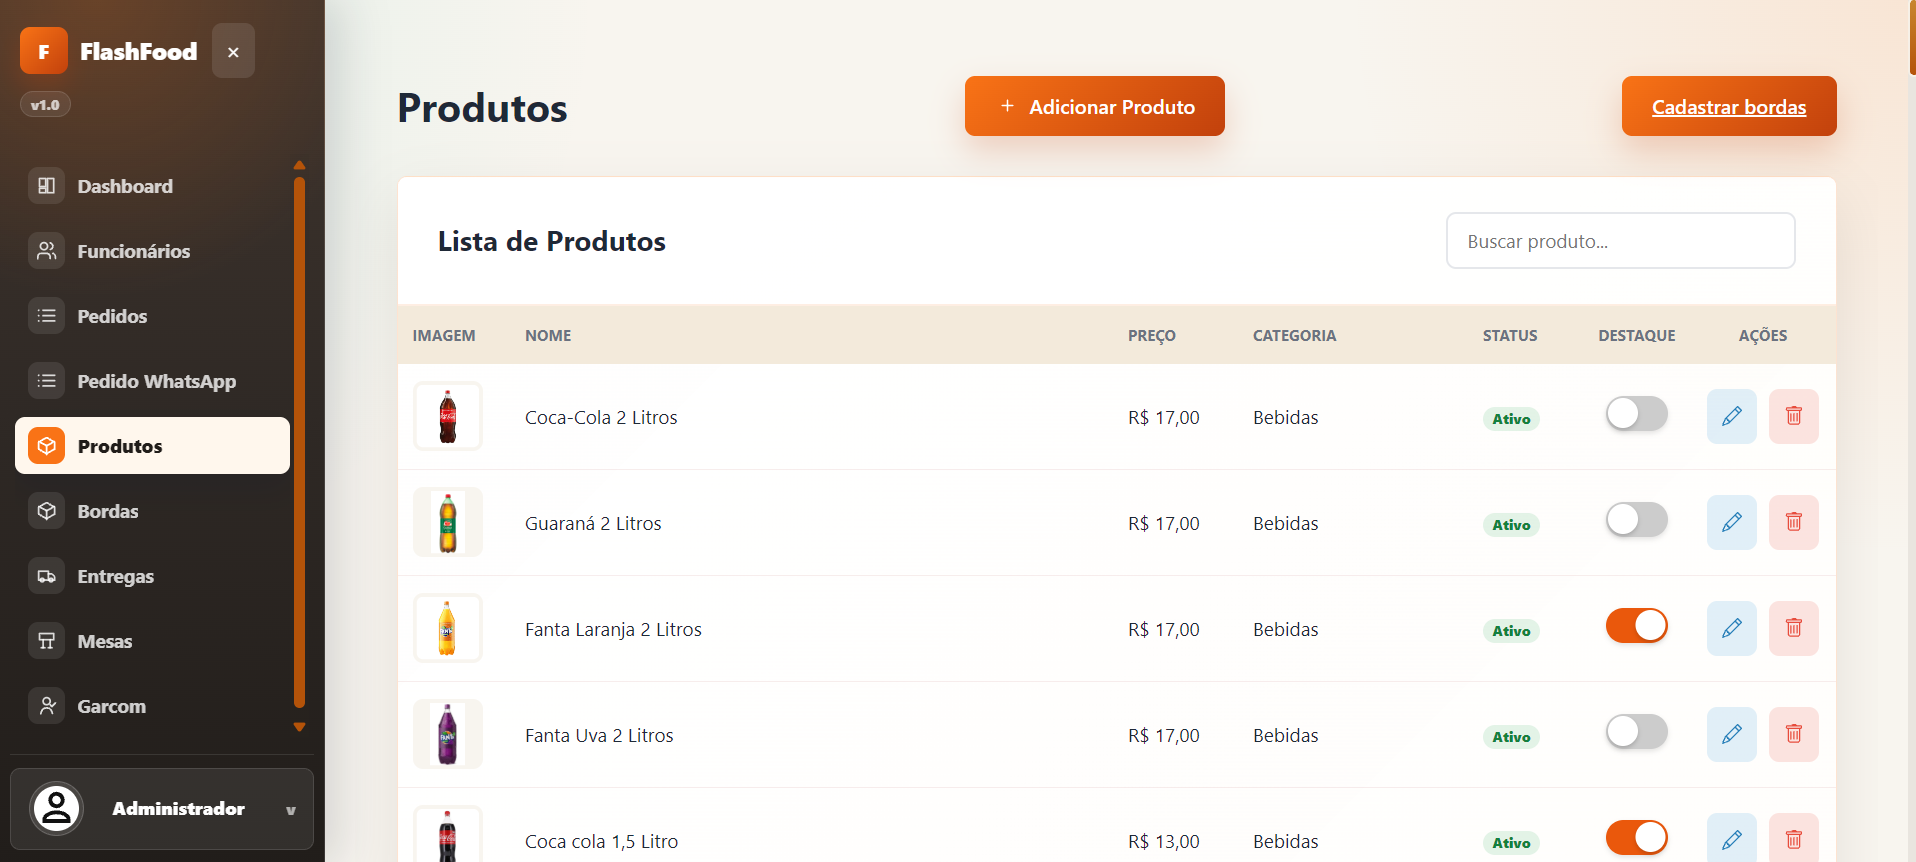
\includegraphics[width=\textwidth,height=0.68\textheight,keepaspectratio]{figuras/captura-cadastro-produto.png}
  \legend{Elaborado pelo autor (2026)}
\end{figure}

A Figura~\ref{fig:permissoes-perfil} apresenta a organização de permissões por grupo de usuários. A tela representa o controle de acesso relacionado ao RF03.

\begin{figure}[H]
  \centering
  \caption{Definição de permissões por perfil}
  \label{fig:permissoes-perfil}
  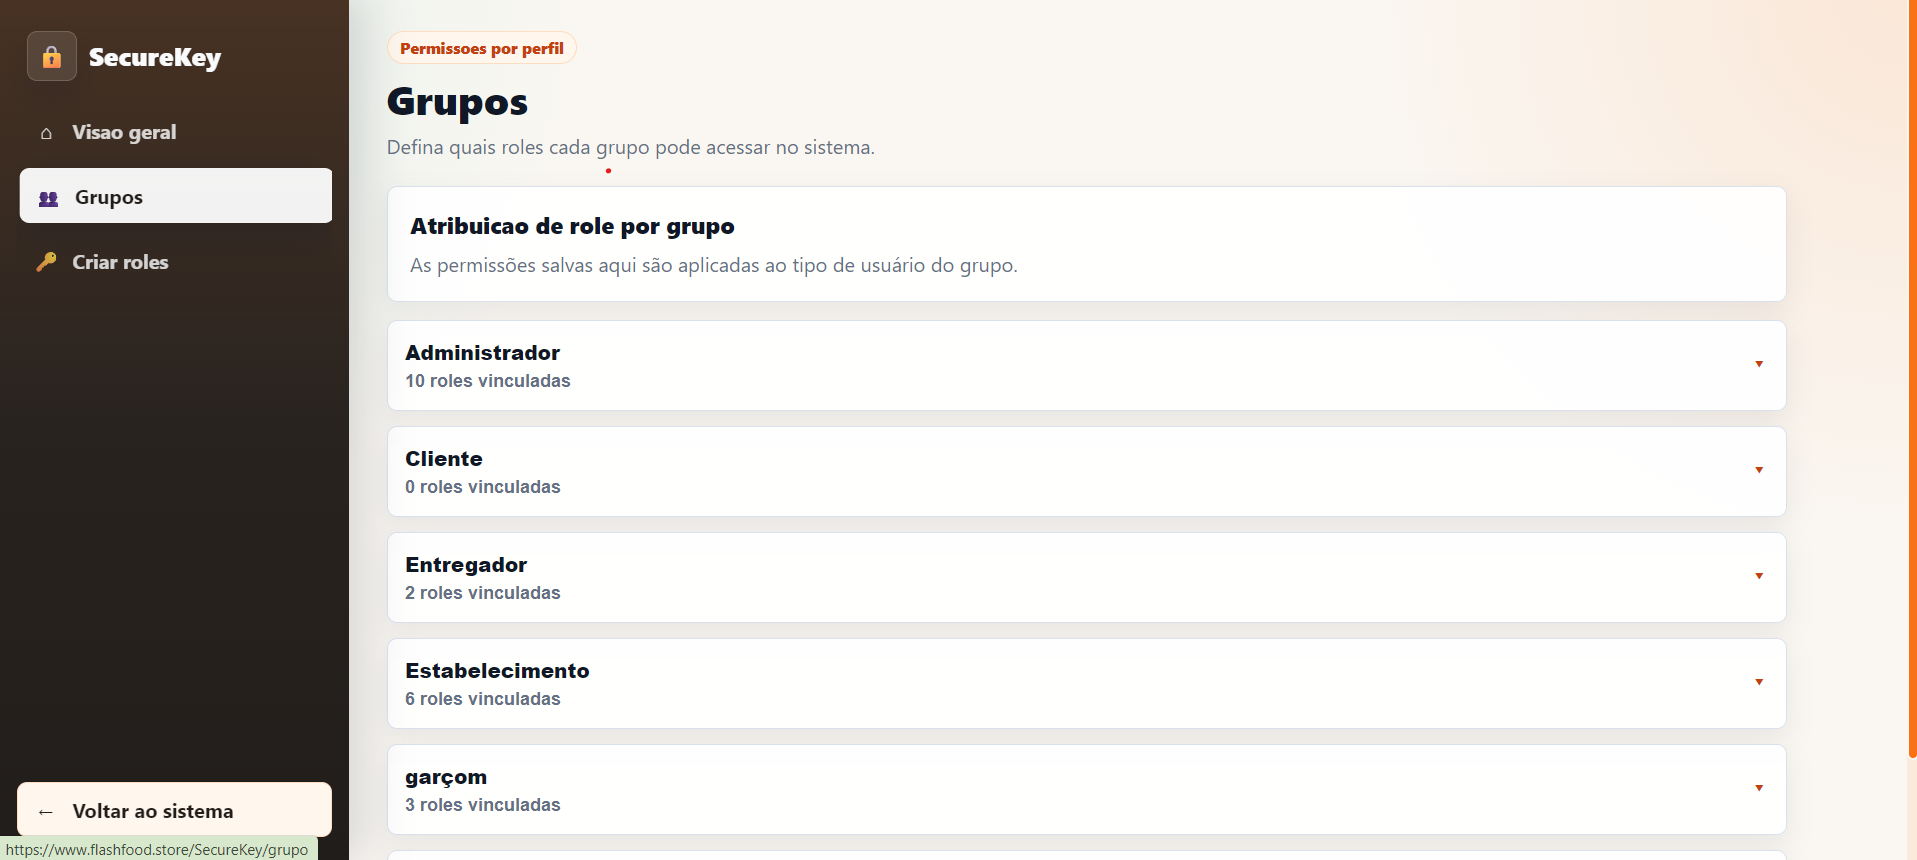
\includegraphics[width=\textwidth,height=0.68\textheight,keepaspectratio]{FlashfoodImagemSistema/telaParaDefinicaoRoles.png}
  \legend{Elaborado pelo autor (2026)}
\end{figure}

A Figura~\ref{fig:configuracao-impressao} mostra a tela de configuração de impressão e sua pré-visualização, utilizada na área administrativa. O acesso conforme o perfil de administrador relaciona-se ao RF03.

\begin{figure}[H]
  \centering
  \caption{Configuração de impressão}
  \label{fig:configuracao-impressao}
  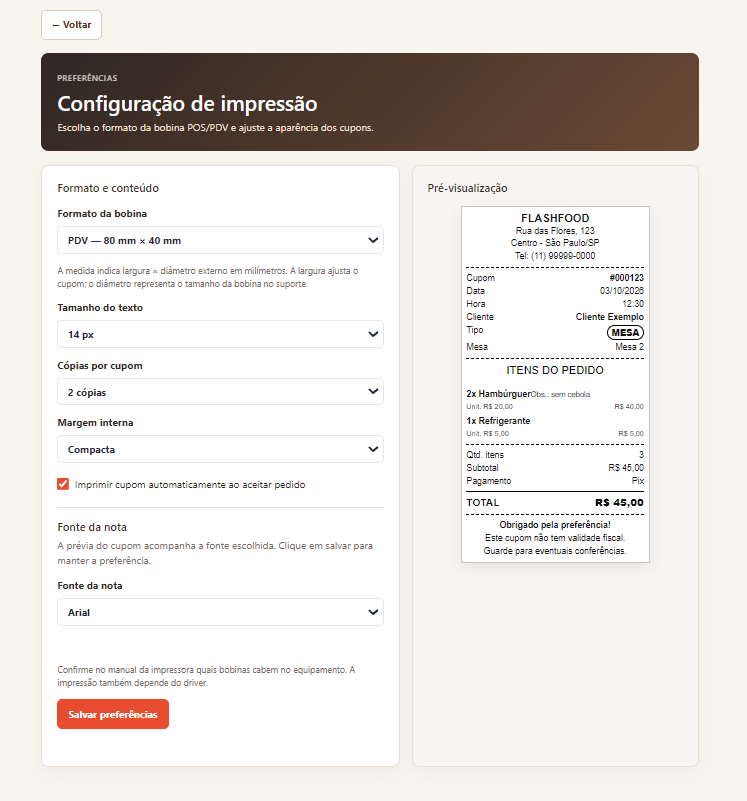
\includegraphics[width=0.9\textwidth,height=0.68\textheight,keepaspectratio]{FlashfoodImagemSistema/telaParaConfiguracaoIMpressao.png}
  \legend{Elaborado pelo autor (2026)}
\end{figure}

\section{Área do funcionário e do garçom}

A Figura~\ref{fig:gerenciamento-mesas} registra a tela de gerenciamento de mesas. Na captura, o perfil exibido é o de administrador; a tela apresenta a situação das mesas e o acesso ao histórico, sendo relacionada ao gerenciamento de pedidos do RF04.

\begin{figure}[H]
  \centering
  \caption{Gerenciamento de mesas no FlashFood}
  \label{fig:gerenciamento-mesas}
  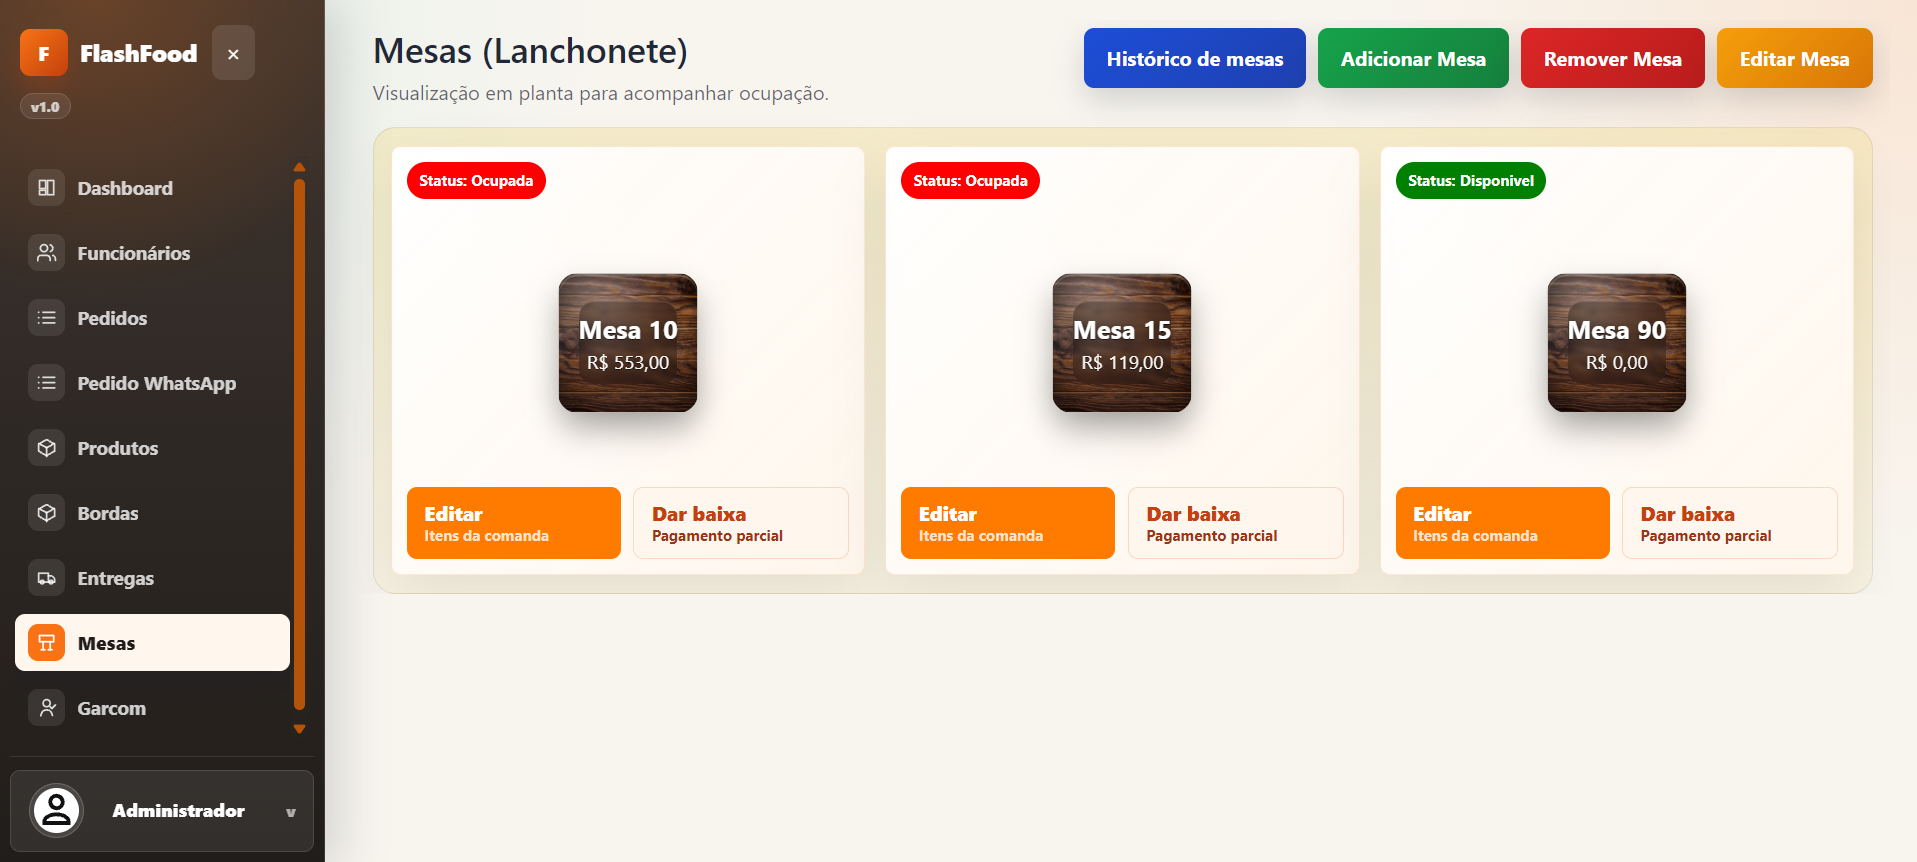
\includegraphics[width=\textwidth,height=0.68\textheight,keepaspectratio]{figuras/captura-gerenciamento-mesa.png}
  \legend{Elaborado pelo autor (2026)}
\end{figure}

\section{Experiência em dispositivos móveis}

A Figura~\ref{fig:cardapio-mobile} apresenta a versão do cardápio em dispositivo móvel e a navegação lateral aberta. As telas são utilizadas pelo cliente para consultar os produtos, atendendo ao RF05.

\begin{figure}[H]
  \centering
  \caption{Cardápio em dispositivo móvel: (a) consulta de produtos; (b) menu de navegação aberto}
  \label{fig:cardapio-mobile}
  \begin{minipage}[t]{0.44\textwidth}
    \centering
    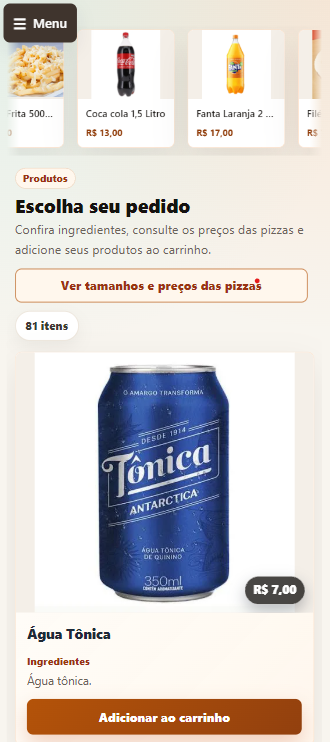
\includegraphics[width=0.85\linewidth,height=0.55\textheight,keepaspectratio]{FlashfoodImagemSistema/mobile.png}
    \par\small (a)
  \end{minipage}\hfill
  \begin{minipage}[t]{0.44\textwidth}
    \centering
    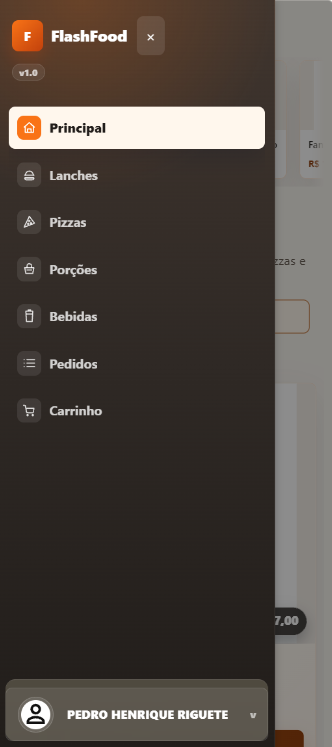
\includegraphics[width=0.85\linewidth,height=0.55\textheight,keepaspectratio]{FlashfoodImagemSistema/menu_mobile.png}
    \par\small (b)
  \end{minipage}
  \legend{Elaborado pelo autor (2026)}
\end{figure}
